\chapter{Building Characteristic Sampling}

There are three steps to creating the sample of buildings modeled by ComStock. The first step creates estimates of the sizes, ages, types, and locations of the buildings that exist throughout the United States.  The second step is characteristic estimation, which is detailed in Section~\ref{chap:4_modeling}. This step defines the additional characteristics of buildings that determine energy consumption and performance. These characteristics are mostly derived from different data sources than those used in the stock estimation step, although they often depend on stock estimation parameters such as building type or age. The third step is sampling the multidimensional probability space to generate a collection of input parameters, or samples. The final samples give an accurate estimation of the commercial building stock at large while not attempting to model any individual building exactly. Stock estimation and sampling are described further in this section, but the majority of the characteristics are discussed in Section~\ref{chap:4_modeling}.

\section{Stock Estimation}

Any estimate of the energy consumption of the U.S. commercial building stock relies heavily on an estimate of how much floor area of each type of building exists in each part of the country. As shown by CBECS \citep{eia2012cbecs} and others, energy consumption of commercial buildings predominantly scales with floor area, not with building count. An accurate estimate of building floor area is therefore a critical input into any stock modeling tool focused on energy or energy-related metrics.

A secondary issue is the type of building associated with each floor area. Although accurately estimating the total floor area of commercial buildings is necessary, it is not sufficient, as building type also has an impact on energy use intensity (EUI), measured in units of energy use per square foot per year. As an example, a large office with a data center would be expected to have a dramatically higher electric load per square foot than an unconditioned warehouse.

The goal of the stock estimation process is to identify the type, floor area, and location of buildings across the United States. This task is complicated by a number of factors, including data sources that are inconsistent across the United States. However, floor area estimation is central to ensuring that ComStock is accurate for its intended use cases. ComStock takes a three step approach towards achieving an accurate estimate. To begin, national data sources are assembled to present overlapping (and often conflicting) reports of the U.S. commercial building stock. Second, the buildings reported by the various data sources are assigned a consistent set of type descriptors---e.g., large office or secondary school. Finally, the various data sets are amalgamated to create a final, consistent data set that is used in the sampling process.

\subsection{Data Sources}

ComStock's stock estimation is assembled using several data sources. The primary data sources are CoStar, a commercial building real estate intelligence broker, and Homeland Infrastructure Foundation-Level Data (HIFLD), a Department of Homeland Security database that provides cross-agency information on critical infrastructure assets across the United States. Both of these data sets, due to their business-/mission-driven use cases, tend to have very high accuracy for the buildings they represent. However, the major downside of both data sources is that the buildings they do not collect data on are not represented in any manner. While this is challenging, it is easier to adjust/correct for this sparsity than to use other data sets in which buildings are incorrectly and inconsistently represented.

CoStar is a ``leading provider of commercial real estate data and marketplace listing platforms. Its data offerings contain in-depth analytical information on over five million commercial real estate properties related to various subsections, including office, retail, multifamily, healthcare, industrial, self-storage, and data centers'' \citep{costar_10k}. CoStar's data is driven by commercial leases and commercial sales data, and is updated with millions of dollars' worth of research per year. CoStar's data set is not always complete, both in terms of geography and building type. For example, building types that are rarely bought and sold, such as schools and major hospital complexes, are less likely to be represented in CoStar's database.

HIFLD is a set of data tables assembled by the U.S. Department of Homeland Security to support critical infrastructure awareness, disaster recovery, and various other uses. Their databases include information on critical infrastructure facilities such as refineries and military bases, but also include information on schools (which are often used as disaster assistance centers) and hospitals. This is particularly useful, as these are two of the key building types that are less likely to be represented in CoStar. Although the schools data set provided by HIFLD always provides information on the number of students enrolled in a given school (which is used as a proxy to determine the floor area of the school when not otherwise available), the hospital table fails to report the number of beds in a given hospital (which is likewise used to scale floor area) in approximately half the states in the United States. In these cases, data from states that do report this information is generalized and used to infer the floor area in states without data.

Although both of these data sets provide excellent coverage of buildings they consider, they do not provide full and complete coverage of commercial buildings across the United States. Of particular note, using these two data sources results in an estimate of U.S. commercial buildings that differs from that published by CBECS. The ComStock team, after significant discussion, has decided to treat the CBECS estimate of the floor area of each building type as a truth data set. Following the sampling of the CoStar and HIFLD data sets, the CBECS estimates are used to ``true up'' the numbers on a national basis. As a result, ComStock's floor area estimates match CBECS' by building type on a national basis. Although other truth data sources were considered, CBECS' centrality to all commercial energy use estimation made it the obvious and consistent choice for estimating the U.S. commercial building stock's energy use.

\subsection{Building Type Assignments}

Building type definitions frequently do not match across data sources. This is particularly noticeable in the case of CoStar, CBECS, and DOE prototype buildings data sources. The DOE prototype building models, discussed further in Section~\ref{sec:building_type_meta}, defines specific combinations of space types as ``building types,'' which are then used by ComStock. The building types represented by the DOE prototype building models were decided on during the development of their precursors, the DOE reference building models \citep{doe_reference_buildings}. As such, ``translating'' building types across data sources introduces a layer of complexity. 

ComStock maps the building type definitions from each data source to a specific building type from the DOE prototype buildings to maximize consistency. While these mappings are imperfect, they represent the best efforts of the ComStock team to capture the unique energy-related characteristics of different building types within the modeling framework created and used by DOE over the last 15 years. Table \ref{tab:building_types} shows the mapping from the CoStar building types and HIFLD tables to the DOE prototype buildings, and from the DOE prototype buildings to CBECS' Principal Building Activity Plus.

\begin{table}
\centering
\small
\caption[Building Type Mapping Across Data Sources]{Building Type Mapping Across Data Sources}
\label{tab:building_types}
\begin{tabular}{|p{4.25cm}|p{3.5cm}|p{3.25cm}|p{4.25cm}|}
\hline
\textbf{CoStar Building   Type}                                & \multicolumn{1}{l|}{\textbf{HIFLD Table}}                & \textbf{DOE Prototype and ComStock Building Type}                               & \textbf{CBECS Principle Building Activity Plus }         \\ \hline
Retail:   Bar                                         & \multirow{2}{*}{Not applicable}                 & \multirow{2}{*}{Full service restaurant}  & Restaurant/cafeteria                            \\ \cline{1-1} \cline{4-4} 
Retail: Restaurant                                    &                                                 &                                           & Bar/pub/lounge                                  \\ \hline
\multicolumn{1}{|l|}{Not applicable}                  & \multicolumn{1}{l|}{Healthcare: Hospitals}      & Hospital                                  & Hospital/inpatient health                       \\ \hline
Hospitality: Hotel                                    & \multirow{12}{*}{Not applicable}                & \multirow{2}{*}{Large hotel}              & \multirow{2}{*}{Hotel}                          \\ \cline{1-1}
Hospitality: Hotel casino                             &                                                 &                                           &                                                 \\ \cline{1-1} \cline{3-4} 
Office: Industrial live/work   unit                   &                                                 & \multirow{6}{*}{Office}                   & Administrative/professional office              \\ \cline{1-1} \cline{4-4} 
Office: Office live/work unit                         &                                                 &                                           & Bank/other financial                            \\ \cline{1-1} \cline{4-4} 
Office: Office/residential                            &                                                 &                                           & Government office                               \\ \cline{1-1} \cline{4-4} 
Retail: Bank                                          &                                                 &                                           & Medical office (non-diagnostic)                 \\ \cline{1-1} \cline{4-4} 
Flex                                                  &                                                 &                                           & \multirow{2}{*}{Other office}                   \\ \cline{1-1}
Office: Service                                       &                                                 &                                           &                                                 \\ \cline{1-1} \cline{3-4} 
Health care: Rehabilitation   center                  &                                                 & \multirow{4}{*}{Outpatient}               & \multirow{2}{*}{Medical office (diagnostic)}    \\ \cline{1-1}
Health care: Skilled nursing   facility               &                                                 &                                           &                                                 \\ \cline{1-1} \cline{4-4} 
Office: Medical                                       &                                                 &                                           & \multirow{2}{*}{Clinic/other outpatient health} \\ \cline{1-1}
Health care                                           &                                                 &                                           &                                                 \\ \hline
\multicolumn{1}{|l|}{\multirow{2}{*}{Not applicable}} & \multicolumn{1}{l|}{Education: Public schools}  & \multirow{2}{*}{Primary/secondary school} & Elementary/middle school                        \\ \cline{2-2} \cline{4-4} 
\multicolumn{1}{|c|}{}                                & \multicolumn{1}{l|}{Education: Private schools} &                                           & High school                                     \\ \hline
Retail: Fast food                                     & \multirow{24}{*}{Not applicable}                & \multirow{2}{*}{Quick service restaurant} & \multirow{2}{*}{Fast food}                      \\ \cline{1-1}
General retail: Fast rood                             &                                                 &                                           &                                                 \\ \cline{1-1} \cline{3-4} 
Retail: Department store                              &                                                 & \multirow{4}{*}{Retail}                   & \multirow{2}{*}{Retail store}                   \\ \cline{1-1}
Retail: Freestanding                                  &                                                 &                                           &                                                 \\ \cline{1-1} \cline{4-4} 
Retail: Garden center                                 &                                                 &                                           & \multirow{2}{*}{Other retail}                   \\ \cline{1-1}
General retail: Freestanding                          &                                                 &                                           &                                                 \\ \cline{1-1} \cline{3-4} 
Hospitality: Motel                                    &                                                 & \multirow{2}{*}{Small hotel}              & \multirow{2}{*}{Motel or inn}                   \\ \cline{1-1}
Hospitality                                           &                                                 &                                           &                                                 \\ \cline{1-1} \cline{3-4} 
Flex: Showroom                                        &                                                 & \multirow{7}{*}{Strip mall}               & \multirow{7}{*}{Strip shopping mall}            \\ \cline{1-1}
Retail: Storefront                                    &                                                 &                                           &                                                 \\ \cline{1-1}
Retail: Storefront   retail/office                    &                                                 &                                           &                                                 \\ \cline{1-1}
Retail: Storefront   retail/residential               &                                                 &                                           &                                                 \\ \cline{1-1}
Specialty: Post office                                &                                                 &                                           &                                                 \\ \cline{1-1}
Retail                                                &                                                 &                                           &                                                 \\ \cline{1-1}
General retail                                        &                                                 &                                           &                                                 \\ \cline{1-1} \cline{3-4} 
Flex: Light distribution                              &                                                 & \multirow{9}{*}{Warehouse}                & \multirow{3}{*}{Distribution/shipping center}   \\ \cline{1-1}
Flex: Light manufacturing                             &                                                 &                                           &                                                 \\ \cline{1-1}
Industrial: Distribution                              &                                                 &                                           &                                                 \\ \cline{1-1} \cline{4-4} 
Industrial: Service                                   &                                                 &                                           & \multirow{3}{*}{Nonrefrigerated warehouse}     \\ \cline{1-1}
Industrial: Showroom                                  &                                                 &                                           &                                                 \\ \cline{1-1}
Industrial: Truck terminal                            &                                                 &                                           &                                                 \\ \cline{1-1} \cline{4-4} 
Industrial: Warehouse                                 &                                                 &                                           & \multirow{3}{*}{Self-storage}                   \\ \cline{1-1}
Specialty: Airplane hangar                            &                                                 &                                           &                                                 \\ \cline{1-1}
Specialty: Self-storage                               &                                                 &                                           &                                                 \\ \hline
\end{tabular}
\end{table}

It is important to note that only one of either the CoStar or HIFLD data is used to represent each type of DOE prototype building---that is, no building type is pulled from both data sets. This ensures that any errors that exist in either data set are independently corrected by the CBECS normalization. According to CBECS' estimation, the amalgamation of these three data sets accounts for 64\% of the energy use and 62\% of the floor area of commercial buildings in the United States. The remaining 36\% of energy use not represented  is due to several CBECS building types that are not included in ComStock yet such as grocery stores and religious worship. Figure \ref{fig:types_not_represented} shows the building types not represented in the ComStock model, on a CBECS Principal Building Activity Plus basis, and their relative contribution to the commercial building energy use in the United States. As can be seen in the figure, college/universities represent the largest un-modeled building classification by energy use, followed by religious institutions, mixed-use offices, grocery stores, nursing homes, and recreational buildings. Although these building types all consume energy, the ComStock team does not have sufficient information to make a reasonable estimate of their energy use, either annually or on a time-series basis, using the approach discussed in Section \ref{sec:space_type_ratios}.

\begin{figure}
  \centering
  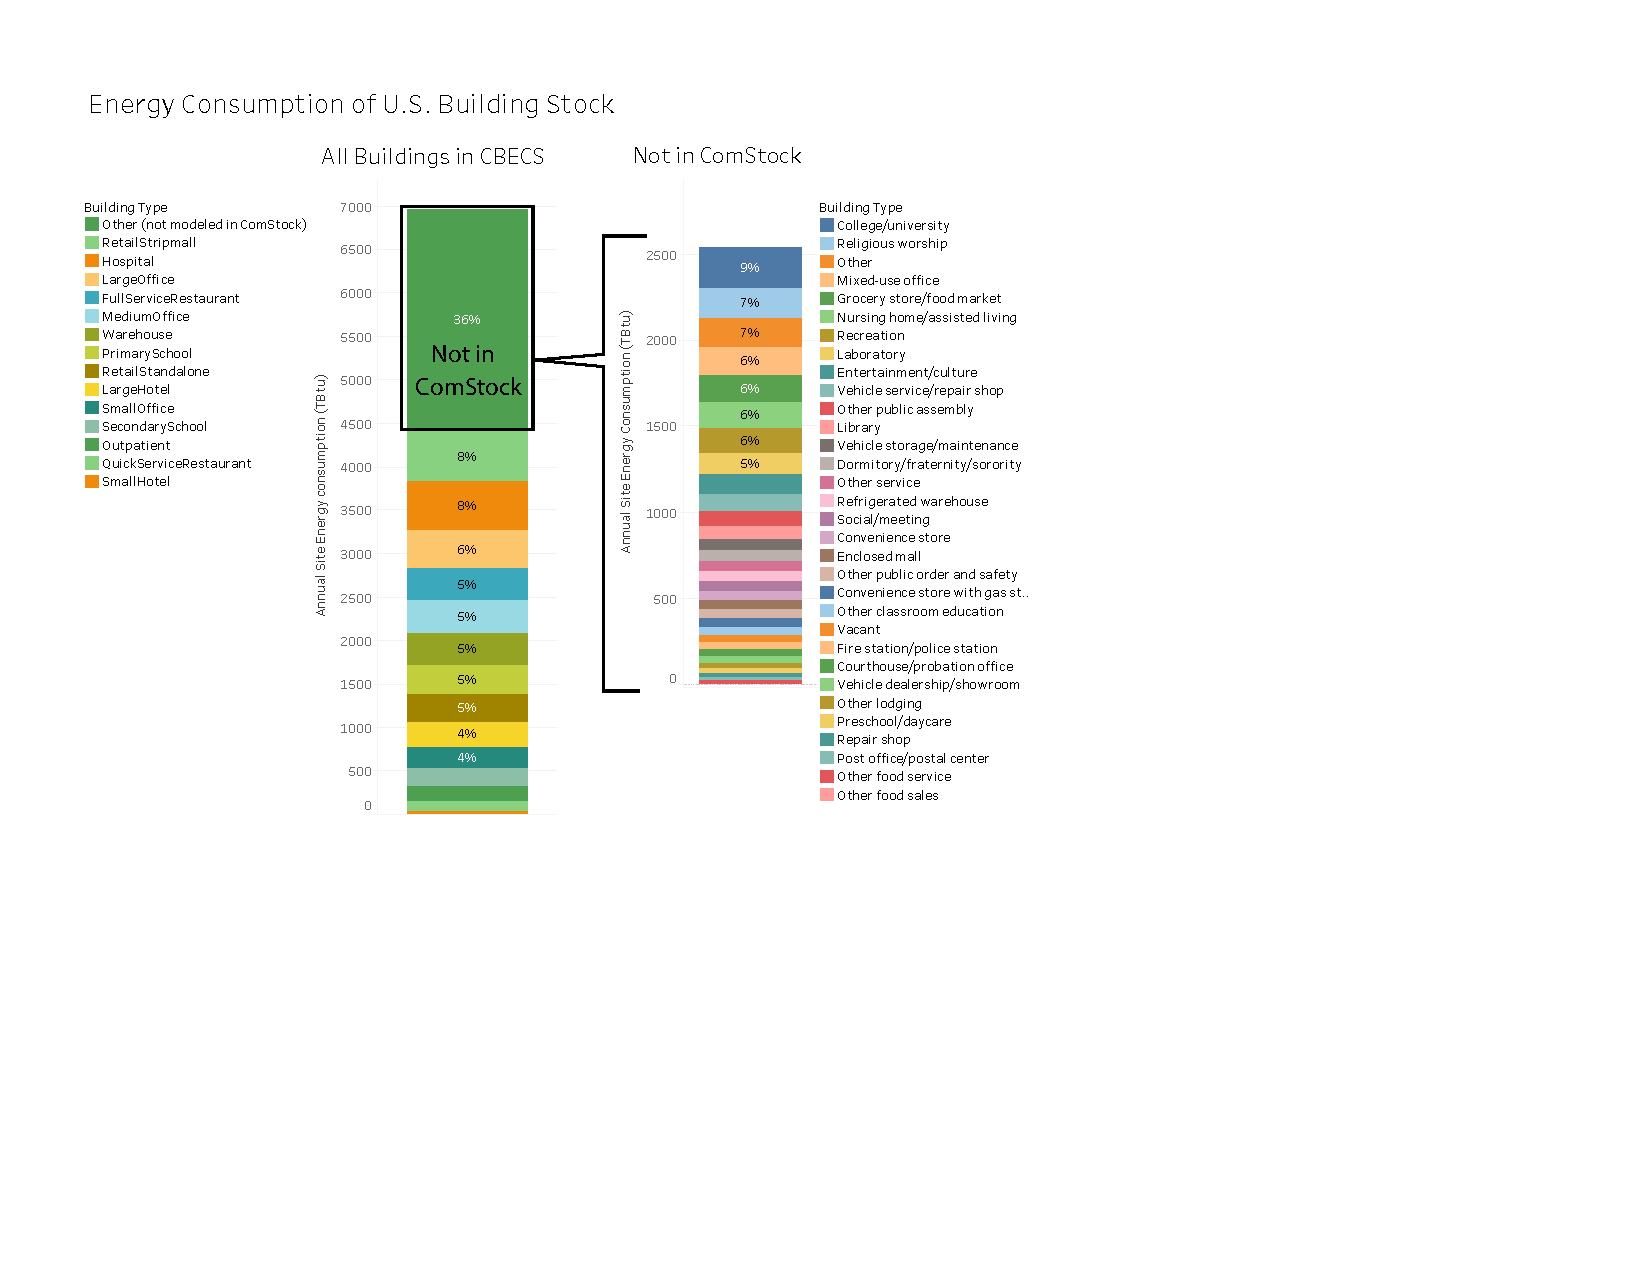
\includegraphics[
        page={1}, 
        trim={1cm 7cm 10cm 1cm}, clip, % L B R T
        width=\textwidth] {figures/CBECS_2012_comstock_coverage.pdf}
  \caption[CBECS building types not covered by ComStock]{CBECS Principal Buildings Activity Plus building types not covered by ComStock on an energy use basis.}
  \label{fig:types_not_represented}
\end{figure}

DOE prototype building type is used to represent a significant amount of the U.S. building stock but is also not used in many cases due to concerns regarding its accurate representation of specific building sub-types. The following list discusses each building type, and what buildings it does and does not represent, as understood by ComStock's developers.

\newpage

\begin{description}
\item [Full Service Restaurant] Both sit-down restaurants and bars are included in this category, as both typically require significant cooking and sanitation equipment for their operation.
\item[Hospital] Hospitals, wherever possible, are disambiguated from outpatient clinics through the existence of around-the-clock medical facilities. This is not possible in many states, in which case the differentiation is based on available CoStar data.
\item[Large Hotel] Large hotels are differentiated from small hotels on the basis of conference or casino spaces. Hotels that have major facilities for conferences, events, or gambling are classified as large hotels.
\item[Offices] Offices are divided up into three subsets: small, medium, and large. Each type of office is based on the thresholds used by American Society of Heating, Refrigerating and Air-Conditioning Engineers (ASHRAE) Appendix G \citep{ashrae_901_2010}, which include both size and number of stories. In the case of large offices, there are additional probability distributions that determine what percent (if any) of the office is a data center.
\item[Outpatient] Outpatient facilities, as represented in ComStock, include non-hospital medical centers, rehabilitation centers, medical offices, and skilled nursing facilities.
\item[Primary School] The primary school type is used to represent all schools that do not include secondary or post-secondary education, i.e., grades 9 and beyond. Schools that provide education for pre-secondary to post-secondary students (e.g., grades 5--12) are classified as secondary schools. This grouping means that any daycare facilities classified as schools by HIFLD are included as primary schools, unless the facilities also support secondary students.
\item[Quick Service Restaurant] Quick service restaurants consist entirely of fast food restaurants.
\item[Retail] This category predominantly features large national retailers, excluding grocery stores. This includes big box stores, garden centers, department stores, and any other freestanding retailers that do not include a significant grocery section.
\item[Secondary School] Secondary schools incorporate all schools that offer instruction to pupils in grades 9--12. No post-secondary institutions (e.g., community colleges and universities) are represented by ComStock unless they fall into another building type defined herein.
\item[Small Hotel] Small hotels encompass all hotels that do not have significant spaces for conferences, meetings, or gambling.
\item[Strip Mall] Strip malls encompass all multi-tenant retail buildings, as well as single-tenant buildings that are not classified as large retailers, such as post offices, showrooms, etc. These buildings have additional probability distributions that determine how much of the building floor area (if any) is a restaurant. This is critically important, as restaurants have a far higher EUI and as a result can cause strip malls to have far higher energy uses than would otherwise be expected in a stand alone retail building.
\item[Warehouse] Warehouses are perhaps the most differentiated building type in the commercial building stock. They are represented in ComStock as a conjunction of office spaces and high-bay spaces. This building type is used to model distribution centers, light manufacturing, and some showroom and truck terminal spaces, as well as airplane hangars, service depots, and self-storage centers. The spaces encompass a large number of functions; however, it is difficult to differentiate these spaces when examining national databases of building stock characteristics. This makes further disambiguation of these buildings impossible without additional data sources.
\end{description}

\subsection{Data Amalgamation for Sampling} \label{sec:3.1.3data amalgamation for sampling}

The data from CoStar and HIFLD were converted from individual building data points to probability distributions for geographic areas due to data retention clauses. 

The ComStock team tagged all individual buildings with a climate zone and a county to convert the county-level locations of buildings within the United States into a probability distribution. From this data, one distribution was created: the likelihood of a building in the United States being located in a given climate zone. In this distribution, there is a much higher likelihood of being located in a heavily populated climate zone (like 4A, which includes much of NJ, DC, MD, DE, VA, etc.) than a sparsely populated climate zone (like 8, which includes only part of AK). Next, for each climate zone, another distribution was created: the likelihood of a building being located in each county within that climate zone. In these distributions, there is a much higher likelihood of being located in a heavily populated county than a sparsely populated county. These two sets of distributions allow any ComStock sample to be assigned a climate zone and a county  prior to any additional characteristics being calculated.

The next characteristic to be described as a probability distribution was the building type. Based on the combined CoStar and HIFLD data sets, the likelihood of a building being of a specific building type was calculated for each county in the United States. In some cases, the county in question had an insufficient number of buildings in CoStar and HIFLD to create a realistic distribution. In these cases, the county was instead assigned a distribution of building types based on all the buildings in the state. This is not frequently required for building type, but is more common for floor area, vintage, and number of stories (discussed next).

Probability distributions for three additional characteristics were created using the HIFLD and CoStar data sets: floor area, vintage, and number of stories. CoStar's database has excellent coverage of floor area of a building as a function of county and building type, good coverage of vintage (the year the building was constructed), and reasonable coverage of the number of stories. HIFLD, on the other hand, has good information on vintage, but not on floor area or the number of stories. For floor area, inferences were based on the number of students enrolled (for schools) and the number of beds (for hospitals). Where information on the number of beds was missing, the aggregate distribution for the United States was used to infer the floor area. The number of stories was estimated based on the inferred floor area for each hospital/school. These estimates, as well as the estimates provided by the CoStar data, were used to create distributions for each building type's characteristics on a county basis. There were several cases in which one or more characteristics could not be accurately estimated for a building type/county pair. In these cases, the aforementioned approach of using the state-level distribution was employed.

The approach employed is mathematically accurate. However, the downside to using building count when creating probability distributions is that a high sample count is required to ensure that less common but highly impactful buildings, such as buildings over one million square feet, are well represented. For example, if a county contains 100 retail stores with a floor area of 1,000 square feet each (for a total of 100,000 square feet) and one retail store (perhaps a mall) of one million square feet, the large retail store would be expected to use roughly ten times (1,000,000 square feet/ 100,000 square feet) the energy of all of the smaller retail stores put together. With the current count-based approach, around 100 samples would need to be generated from this distribution to ensure that the one million square foot retail store was represented in the model. Although the impacts of this are minimal at a higher geographic level, it is a known weakness of the current approach.

\section{Characteristic Estimation} \label{Characteristic Estimation}

The variability of the commercial building stock begins with building type and location, but extends to include a variety of additional factors. These include schedule diversity, installed equipment type, age of installed equipment, and building code. Each of the characteristics associated with these categories are discussed at length in Section \ref{chap:4_modeling}, and overviews of each are provided below.

Schedule diversity is a key source of variability in the U.S. commercial building stock. Some buildings operate on a 24/7 basis, but the percentage varies drastically by building type---i.e., there are very few primary schools throughout the United States that are ``on'' 24 hours per day, let alone 365 days per year. There is also monthly/seasonal variability in a few building types, most notably schools and hotels. Although many of the buildings have lower occupant- or schedule-driven loads during various periods, some do not (e.g., schools that offer summer school). The nuances of this variability are represented in the schedule-driven characteristic distributions.

Equipment characteristics can make a significant difference in the energy consumption of a building through differences in efficiency, fuel type, and the presence or absence of certain types of equipment. ComStock represents this variability by accounting for the fuel type variability within a given state. This allows ComStock to calculate the likelihood of various heating, ventilating, and air-conditioning (HVAC) system types as a function of building type and fuel type. As part of this calculation, systems that do not provide cooling are considered, particularly in the case of warehouses. The fuel type distribution is also used as an input to the selection of water heating equipment.

The third major category of variability is equipment vintage. In most cases, this category is driven by the age of the building. Equipment within a building is generally updated and replaced over time for reasons such as remodeling or equipment failure. As discussed in Section~\ref{sec:system_turnover_and_eul}, there is a great degree of variability in equipment lifespans, which leads to variability in the current equipment installed in buildings of a given year of construction. The age of the equipment (or, put another way, the year of manufacture/sale of the equipment) plays a large part in a buildings' efficiency. In some cases, such as buildings built within the last 5--10 years, it is unlikely that many of the building systems have been replaced. The equipment distribution, which is conditioned on the building's year of construction, reflects these nuances.

Finally, building energy codes have an impact on the efficiency of components installed within a building. Building energy codes set the minimum efficiency levels for various building components, but code adoption is not uniform across the United States. As discussed in Section~\ref{sec:energy_code}, the building code in force at the time of replacement/installation of a building component is a key driver of its efficiency.

\section{Publication of Building Characteristic Probability Distributions}
Some of the distributions described above cannot be published for contractual agreement reasons, but certain distributions can be published. The ComStock team has generated tab-separated values (tsv) files containing probabilities and dependencies. See Table \ref{tbl:distro_tbl} for the full list of building characteristic probability distributions. More detail on each building characteristic is provided later in this report.

\begin{center}
\small
\begin{longtable}{|p{1.3in}|p{1.5in}|p{1.5in}|p{1.5in}|}
\caption[Building Characteristic Distributions]{Building Characteristic Distributions Included in the ComStock Sampling Process, Including Probabilistic Dependencies and Descriptions} \\ \hline
\label{tbl:distro_tbl}
\textbf{Building Characteristic} & \textbf{Description} & \textbf{Data Source} & \textbf{Conditional On} \\ \hline
\endfirsthead
\multicolumn{4}{c} {{\bfseries \textit{Continued from previous page}}} \\ \hline
\textbf{Building Characteristic} & \textbf{Description} & \textbf{Data Source} & \textbf{Conditional On} \\ \hline
\endhead
Simulation Year                                                 & Year used in simulations                                                       &                                                            &                                                                                                      \\ \hline
Climate Zone                                                    & Climate zone as defined by American Society of Heating, Refrigerating and Air-Conditioning Engineers (ASHRAE) Standard 169--2006                            & CoStar                                                      &                                                                                                      \\ \hline
County                                                          & County FIPS code (includes state specification)                                & CoStar                                                      & Climate Zone                                                                                         \\ \hline
State                                                           & State FIPS code                                                                & CoStar                                                      & County                                                                                               \\ \hline
Building Type                                                   & Primary building type of model                                                 & CoStar                                                      & County                                                                                               \\ \hline
Building Rentable Area                                          & Building total floor area                                                      & CoStar                                                      & County, Building Type                                                                                \\ \hline
Census Region                                                   & Census region                                                                  & CoStar                                                      & State                                                                                                \\ \hline
Year of Construction                                            & Year in which the building was constructed                                     & CoStar                                                      & County, Building Type, Simulation Year                                                               \\ \hline
Year of Construction Bin                                        & Year bin in which the building was constructed                                 & CPUC DEER EULs                                              & Year of Construction                                                                                 \\ \hline
Energy Code in Force When Constructed                           & Energy code applicable to building when constructed                            & State Code Adoption History                                 & State, Year of Construction Bin                                                                      \\ \hline
Building Subtype                                               & If applicable, subtype of primary building type                                & NREL analysis of strip malls                                & Building Type                                                                                        \\ \hline
Ownership Status                                                & Ownership and occupant status of the building                                  & CBECS 2012                                                  & Building Type                                                                                        \\ \hline
Party Responsible for Purchase Authority                        & Entity responsible for purchasing decisions                                    & CBECS 2012                                                  & Ownership Status                                                                                     \\ \hline
Party Responsible for Operation                                 & Entity responsible for operation of the building                               & CBECS 2012                                                  & Ownership Status                                                                                     \\ \hline
Number of Stories                                               & Number of stories above grade                                                  & CoStar                                                      & County, Building Type                                                                                \\ \hline
Window-to-Wall Ratio                                            & Window-to-wall ratio                                                           & NFRC Commercial Fenestration Market Study                   & Building Type, Building Rentable Area, Energy Code in Force When Constructed                         \\ \hline
Building Shape                                                  & Building shape designation                                                     & CBECS 2012                                                  & Building Type                                                                                        \\ \hline
Aspect Ratio                                                    & Aspect ratio of building                                                       & CBECS 2012                                                  & Building Shape                                                                                       \\ \hline
Building Rotation                                               & Rotation of building relative to North                                         & CBECS 2012                                                  &                                                                                                      \\ \hline
Space Heating Fuel                                              & Principal heating fuel for the building                                        & CBECS 2012 Plus ResStock Residential Heating Fuel by County & Building Type, County                                                                                \\ \hline
Water Heating Fuel                                              & Heating fuel for service water heating                                         & CBECS 2012~                                                 & Space Heating Fuel, Building Type                                                                    \\ \hline
HVAC System Type                                                & Primary building HVAC system type                                              & CBECS                                                       & Building Type, Space Heating Fuel, Census Region                                                     \\ \hline
HVAC Nighttime Variability                                      & HVAC nighttime ventilation operation                                           & NREL end-use data analysis                                  & HVAC System Type, Building Type                                                                      \\ \hline
Weekday Operation Start Time                                    & Building weekday operation start time                                          & NREL/Lawrence Berkeley National Laboratory (LBNL) AMI analysis                                      & Building Type                                                                                        \\ \hline
Weekend Operation Start Time                                    & Building weekend operation start time                                          & NREL/LBNL AMI analysis                                      & Building Type                                                                                        \\ \hline
Weekday Operational Duration                                    & Building weekday operation duration                                            & NREL/LBNL AMI analysis                                      & Building Type, Weekday Operation Start Time                                                          \\ \hline
Weekend Operational Duration                                    & Building weekend operation duration                                            & NREL/LBNL AMI analysis                                      & Building Type, Weekend Operation Start Time                                                          \\ \hline
Thermostat Set point for Heating                                 & Heating set point during occupied hours                                         & NREL Tstat data analysis                                    & Building Type                                                                                        \\ \hline
Thermostat Setback for Heating                                  & Heating setback during unoccupied hours                                        & NREL Tstat data analysis                                    & Building Type                                                                                        \\ \hline
Thermostat Set point for Cooling                                 & Cooling set point during occupied hours                                         & NREL Tstat data analysis                                    & Building Type                                                                                        \\ \hline
Thermostat Setback for Cooling                                  & Cooling setback during unoccupied hours                                        & NREL Tstat data analysis                                    & Building Type                                                                                        \\ \hline
Wall Construction Type                                          & Building wall construction type                                                & LightBox                                                    & Climate Zone, Number of Stories                                                                      \\ \hline
Lighting Technology Size Bin                                    & Building size classification for lighting technology type                      &                                                             & Building Rentable Area                                                                               \\ \hline
Plug Load Base-to-Peak Ratio type                                & Methodology for variability of plug load amplitude                              & NREL end-use data analysis                                  & Building Type                                                                                        \\ \hline
Plug Load Weekday Base-to-Peak Ratio                             & Ratio between nominal and maximum weekday plug Load levels                      & NREL end-use data analysis                                  & Building Type, Plug Load Base-to-Peak Ratio Type                                                      \\ \hline
Plug Load Weekend Base-to-Peak Ratio                             & Ratio between nominal and maximum weekend plug Load levels                      & NREL end-use data analysis                                  & Building Type, Plug Load Base-to-Peak Ratio Type                                                      \\ \hline
Lighting Base-to-Peak Ratio Type                                & Methodology for variability of lighting load amplitude                         & NREL end-use data analysis                                  & Building Type                                                                                        \\ \hline
Lighting Weekday Base-to-Peak Ratio                             & Ratio between nominal and maximum weekday lighting load levels                 & NREL end-use data analysis                                  & Building Type, Lighting Base-to-Peak Ratio Type                                                      \\ \hline
Lighting Weekend Base-to-Peak Ratio                             & Ratio between nominal and maximum weekend lighting load levels                 & NREL end-use data analysis                                  & Building Type, lighting Base-to-Peak Ratio Type                                                      \\ \hline
Code Compliance for Building Construction                       & Building energy code compliance when first constructed                         & Assumption                                                  & State                                                                                                \\ \hline
Code Compliance for Interior Lighting                           & Building energy code compliance for latest interior lighting replacement       & Assumption                                                  & State                                                                                                \\ \hline
Code Compliance for Walls                                       & Building energy code compliance for latest walls replacement                   & Assumption                                                  & State                                                                                                \\ \hline
Code Compliance for Service Water Heating                       & Building energy code compliance for latest service water heating replacement   & Assumption                                                  & State                                                                                                \\ \hline
Code Compliance for Roof                                        & Building energy code compliance for latest roof replacement                    & Assumption                                                  & State                                                                                                \\ \hline
Code Compliance for Exterior Lighting                           & Building energy code compliance for latest exterior lighting replacement       & Assumption                                                  & State                                                                                                \\ \hline
Code Compliance for Interior Equipment                          & Building energy code compliance for latest interior equipment replacement      & Assumption                                                  & State                                                                                                \\ \hline
Code Compliance for Windows                                     & Building energy code compliance for latest window replacement                  & Assumption                                                  & State                                                                                                \\ \hline
Code Compliance for HVAC                                        & Building energy code compliance for latest HVAC replacement                    & Assumption                                                  & State                                                                                                \\ \hline
Last Replacement Year for Interior Lighting                     & Year of most recent replacement of the interior lighting system                & CPUC DEER EULs                                              & Simulation Year, Year of Construction                                                                \\ \hline
Last Replacement Year for HVAC                                  & Year of most recent replacement of the HVAC system                             & CPUC DEER EULs                                              & Simulation Year, Year of Construction                                                                \\ \hline
Last Replacement Year for Service Water Heating                 & Year of most recent replacement of the service water heating system            & CPUC DEER EULs                                              & Simulation Year, Year of Construction                                                                \\ \hline
Last Replacement Year for Walls                                 & Year of most recent replacement of the wall                                    & CPUC DEER EULs                                              & Simulation Year, Year of Construction                                                                \\ \hline
Last Replacement Year for Windows                               & Year of most recent replacement of the windows                                 & CPUC DEER EULs                                              & Simulation Year, Year of Construction                                                                \\ \hline
Last Replacement Year for Roof                                  & Year of most recent replacement of the roof                                    & CPUC DEER EULs                                              & Simulation Year, Year of Construction                                                                \\ \hline
Last Replacement Year for Exterior Lighting                     & Year of most recent replacement of the exterior lighting system                & CPUC DEER EULs                                              & Simulation Year, Year of Construction                                                                \\ \hline
Last Replacement year for Interior Equipment                    & Year of most recent replacement of the interior equipment system               & CPUC DEER EULs                                              & Simulation Year, Year of Construction                                                                \\ \hline
Code in Force for Replacement of Interior Lighting              & Energy code in force at time of last interior lighting renovation              & State Code Adoption History                                 & State, Last Replacement Year for Interior Lighting                                                   \\ \hline
Code in Force for Replacement of Windows                        & Energy code in force at time of last window renovation                         & State Code Adoption History                                 & State, Last Replacement Year for Windows                                                             \\ \hline
Code in Force for Replacement of Roof                           & Energy code in force at time of last roof renovation                           & State Code Adoption History                                 & State, Last Replacement Year for Roof                                                                \\ \hline
Code in Force for Replacement of HVAC                           & Energy code in force at time of last HVAC renovation                           & State Code Adoption History                                 & State, Last Replacement Year for HVAC                                                                \\ \hline
Code in Force for Replacement of Walls                          & Energy code in force at time of last walls renovation                          & State Code Adoption History                                 & State, Last Replacement Year for Walls                                                               \\ \hline
Code in Force for Replacement of Service Water Heating          & Energy code in force at time of last service water heating renovation          & State Code Adoption History                                 & State, Last Replacement Year for Service Water Heating                                               \\ \hline
Code in Force for Replacement of Interior Equipment             & Energy code in force at time of last interior equipment renovation             & State Code Adoption History                                 & State, Last Replacement year for Interior Equipment                                                  \\ \hline
Code in Force for Replacement of Exterior Lighting              & Energy code in force at time of last exterior lighting renovation              & State Code Adoption History                                 & State, Last Replacement Year for Exterior Lighting                                                   \\ \hline
Energy Code Followed for Building Construction                  & Energy code followed when building was constructed                             & State Code Adoption History Plus Year Built and Turnover    & Energy Code in Force when Constructed, Code Compliance for Building Construction                     \\ \hline
Energy Code Followed for Replacement of Interior Lighting       & Energy code followed when current interior lighting system installed           & State Code Adoption History Plus Year Built and Turnover    & Code in Force for Replacement of Interior Lighting, Code Compliance for Interior Lighting            \\ \hline
Energy Code Followed for Replacement of Service Water Heating   & Energy code followed when current service water heating system installed       & State Code Adoption History Plus Year Built and Turnover    & Code in Force for Replacement of Service Water Heating, Code Compliance for Service Water Heating    \\ \hline
Energy Code Followed for Replacement of Windows                 & Energy code followed when current windows were installed                       & State Code Adoption History Plus Year Built and Turnover    & Code in Force for Replacement of Windows, Code Compliance for Windows                                \\ \hline
Energy Code Followed for Replacement of Roof                    & Energy code followed when current roof was installed                           & State Code Adoption History Plus Year Built and Turnover    & Code in Force for Replacement of Roof, Code Compliance for Roof                                      \\ \hline
Energy Code Followed for Replacement of Interior Equipment      & Energy code followed when current interior equipment installed                 & State Code Adoption History Plus Year Built and Turnover    & Code in Force for Replacement of Interior Equipment, Code Compliance for Interior Equipment          \\ \hline
Energy Code Followed for Replacement of HVAC                    & Energy code followed when current HVAC system installed                        & State Code Adoption History Plus Year Built and Turnover    & Code in Force for Replacement of HVAC, Code Compliance for HVAC                                      \\ \hline
Energy Code Followed for Replacement of Walls                   & Energy code followed when current walls were installed                         & State Code Adoption History Plus Year Built and Turnover    & Code in Force for Replacement of Walls, Code Compliance for Walls                                    \\ \hline
Energy Code Followed for Replacement of Exterior Lighting       & Energy code followed when current exterior lighting system installed           & State Code Adoption History Plus Year Built and Turnover    & Code in Force for Replacement of Exterior Lighting, Code Compliance for Exterior Lighting            \\ \hline
Lighting Technology Generation                                  & Generation of lighting technology used in building                             & Lighting Market Characterization                            & Code in Force for Replacement of Interior Lighting, Last Replacement Year for Interior Lighting      \\ \hline
Window Technology Type                                          & Window technology type used in the building                                    & NFRC Commercial Fenestration Market Study                   & Energy Code Followed for Replacement of Windows, Climate Zone                                        \\ \hline
\end{longtable}
\end{center}

\section{Sampling Methodology}
The previous subsections describe the creation of building characteristic probability distributions that are in many cases are conditional on one another. These  distributions, when joined together, create a multidimensional joint probability distribution. This joint probability distribution represents the ComStock team's best estimate of the building characteristics of the commercial building stock in the United States. In order to go from the joint probability distribution to a set of discrete building samples, a sampling algorithm must be used.

Several different classes of algorithms support sampling in multidimensional probability spaces. ComStock's choice has largely been influenced by \cite{sobol_sampling}, which introduced Sobol Sequences as a low-discrepancy basis for sampling in higher-dimensional spaces. This approach attempts, with each sample, to optimally reduce the maximal space between samples. Although this approach can be implemented on an iterative basis, ComStock adopted an approach developed by \cite{sobol_lib}, which uses a bit-switching algorithm to select optimal sampling within an $n$-dimensional probability space. This approach is designed to accurately capture the full extent of the distributions with limited samples on a non-biased basis. In other words, all buildings within a type are equally weighted after sampling, rather than being reweighted as a secondary step to sampling.

The results of applying these algorithms produced 350,000 building samples. The set of characteristics for each sample defines the inputs to the ComStock BEM workflow, which creates a BEM for each sample. The characteristics of the 350,000 samples are recorded in the buildstock.csv file. The buildings described in this file provide the ComStock team's best estimate of the characteristics for a large portion of the United States' commercial building stock for use by researchers, practitioners, and consultants. For a detailed look at the accuracy of the resulting models, refer to \cite{eulp_final_report}. The building energy models for ComStock's 350,000 baseline building samples are available to download at \url{https://data.openei.org/} in the nrel-pds-building-stock data lake. See the README.md file for details.